% Seção 5 — resultados obtidos e discussão; integrada à versão thesis_v3.
\section{Resultados e discussão}
\label{sec:resultados}

\subsection{Parâmetros e ganhos obtidos da síntese}
\label{subsec:resultados_sintese}

Os valores fixos das incognitas do modelo, e os intervalos de operação associados aos parâmetro variáveis, são apresentados na Tabela~\ref{tab:parametros_planta}. As três variáveis incertas consideradas geram oito combinações extremas, identificadas na Tabela~\ref{tab:vertices}.

\begin{table}[htbp]
    \centering
    \caption{Parâmetros utilizados na modelagem da planta farmacocinética.}
    \label{tab:parametros_planta}
    \begin{tabular}{lcc}
        \toprule
        Parâmetro & Valor mínimo & Valor máximo\\
        \midrule
        $\gamma_{ob}$ & $0,037$ & $0,040$\\
        $\mu_m$ & $0,100$ & $0,200$\\
        $\mu_o$ & $0,100$ & $0,150$\\
        \midrule
        \multicolumn{3}{l}{Parâmetros fixos: $\gamma_{mb}=0,095$, $\gamma_{bo}=0,095$, $\gamma_{bm}=0,030$, $\mu_b=0,200$.}\\
        \multicolumn{3}{l}{$D_m=0,010$.}\\
        \bottomrule
    \end{tabular}
\end{table}

\begin{table}[htbp]
    \centering
    \caption{Combinações extremas dos parâmetros incertos utilizadas no MATLAB/Simulink.}
    \label{tab:vertices}
    \begin{tabular}{cccc}
        \toprule
        Vértice & $\gamma_{ob}$ & $\mu_m$ & $\mu_o$\\
        \midrule
        V1 & $0,037$ & $0,10$ & $0,10$\\
        V2 & $0,037$ & $0,10$ & $0,15$\\
        V3 & $0,037$ & $0,20$ & $0,10$\\
        \textbf{V4} & $\mathbf{0,037}$ & $\mathbf{0,20}$ & $\mathbf{0,15}$\\
        \textbf{V5} & $\mathbf{0,040}$ & $\mathbf{0,10}$ & $\mathbf{0,10}$\\
        V6 & $0,040$ & $0,10$ & $0,15$\\
        V7 & $0,040$ & $0,20$ & $0,10$\\
        V8 & $0,040$ & $0,20$ & $0,15$\\
        \bottomrule
    \end{tabular}
\end{table}

A aplicação do procedimento iterativo de síntese, descrito na Subseção~\ref{subsec:lmis}, forneceu os seguintes ganhos para o controlador PI:
\begin{equation}
    \boxed{K_p=-16,6825,\qquad K_i=2,2578.}
    \label{eq:ganhos_pi_resultado}
\end{equation}

\subsection{Resultados da simulação em MATLAB/Simulink}
\label{subsec:resultados_simulink}

Através de Simulink, simulou-se a malha de controle fechada para os oito vértices apresentados na Tabela~\ref{tab:vertices} e agruparam-se os resultados na Figura~\ref{fig:respostas_vertices_simulink}. Nas simulações usou-se uma referência constante $r(k)=15$, com um período de amostragem configurado em $T_s=0,01\,\mathrm{s}$, um intervalo de simulação de $7\,\mathrm{s}$, com os ganhos do controlador configurados como apresentado na Equação~\eqref{eq:ganhos_pi_resultado}.

\begin{figure}[htbp]
    \centering
    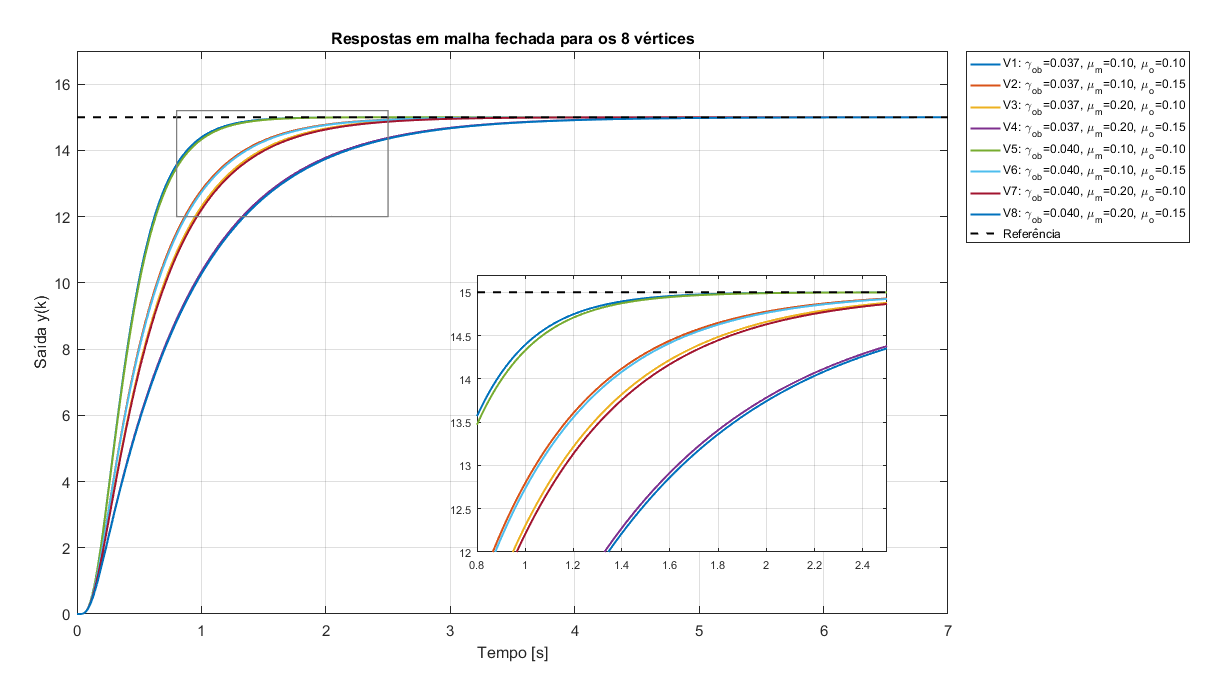
\includegraphics[width=\textwidth]{resposta_simulink_simulacao.png}
    \caption{Respostas da malha fechada para os oito vértices, considerando uma referência fixa de $r(k)=15$.}
    \label{fig:respostas_vertices_simulink}
\end{figure}

Observa-se que, para todas as combinações extremas avaliadas, a saída se aproxima da referência sem sobressinal perceptível no gráfico. Dependo do parâmetro variado, as curvas apresentam velocidades de resposta distintas e algumas delas ficam próximas, pelo qual uma região da figura foi ampliada.

\subsection{Resultados da emulação embarcada}
\label{subsec:resultados_embarcados}

A dashboard desenvolvida através de Node-Red e FlowFuse pode ser visualizada na Figura~\ref{fig:dashboard_nodered}. Nela, registraram-se diversas informações do sistema em tempo real, como: o vetor de estados expandido, os parametros variáveis da planta, o sinal de controle ($u(k)$), a saída ($y(k)$) e a referência ($r(k)$).

\begin{figure}[htbp]
    \centering
    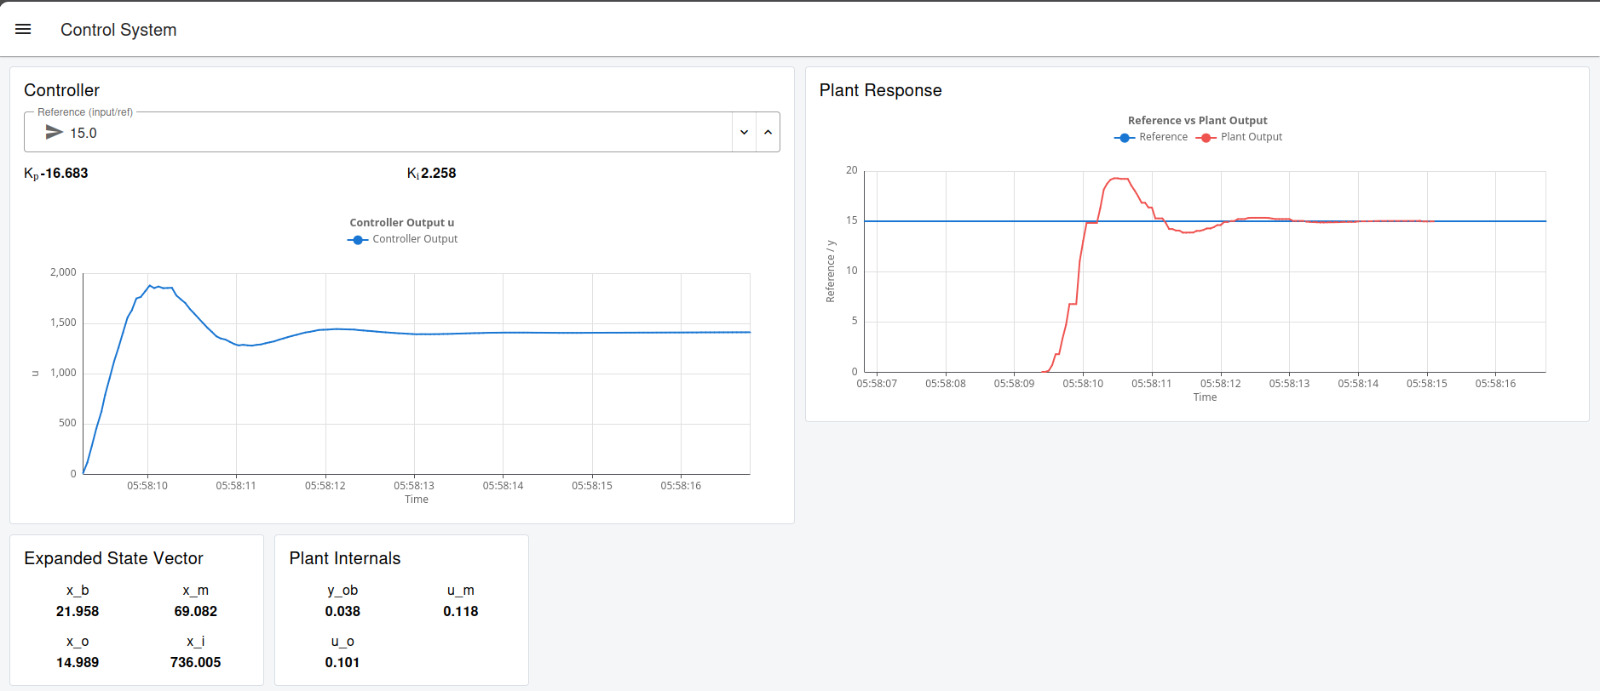
\includegraphics[width=.96\textwidth]{dashboard_nodered.jpg}
    \caption{Dashboard desenvolvida com Node-RED e FlowFuse Dashboard para ajuste da referência e supervisão da malha de controle.}
    \label{fig:dashboard_nodered}
\end{figure}

Para comparar diferentes condições de operação, foram selecionados os vértices V4 e V5 do politopo, cujos valores constam da Tabela~\ref{tab:vertices}. Em cada teste os outros parâmetros do modelo permaneceram inalterados e, para cada vértice, variou-se a referência de 0 para 15 e de 15 para 0. Nas Figuras \ref{fig:ensaio_v4} e \ref{fig:ensaio_v5} podem ser visualizados os gráficos comparativos de referência e saída, com o objetivo de mostrar o rastreamento da referência nas condições de operação já descritas.

\begin{figure}[htbp]
    \centering
    \begin{subfigure}{0.95\textwidth}
        \centering
        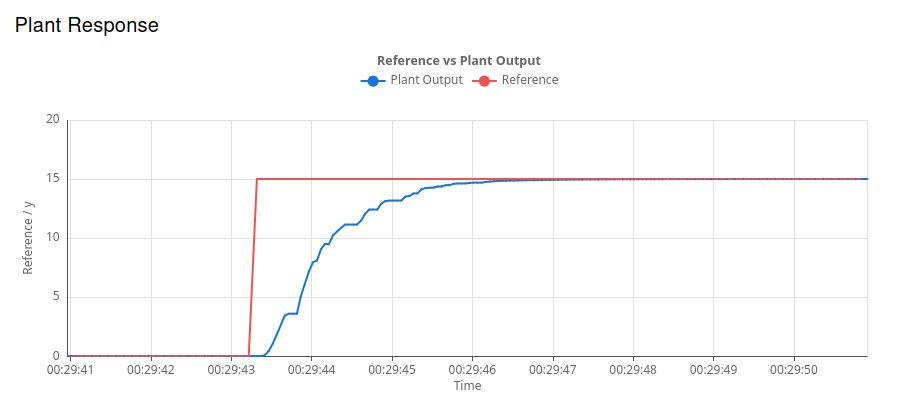
\includegraphics[width=\linewidth]{ensaio_v4_subida_planta.png}
        \caption{Alteração da referência de 0 para 15.}
    \end{subfigure}
    \vspace{0.3cm}
    \begin{subfigure}{0.95\textwidth}
        \centering
        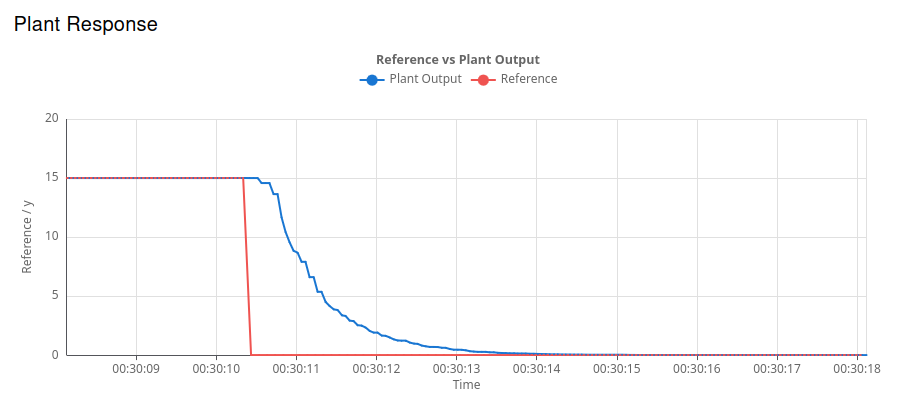
\includegraphics[width=\linewidth]{ensaio_v4_descida_planta.png}
        \caption{Alteração da referência de 15 para 0.}
    \end{subfigure}
    \caption{Rastreamento da referência na plataforma embarcada para o vértice V4 ($\gamma_{ob}=0,037$, $\mu_m=0,20$ e $\mu_o=0,15$). Capturas do Node-RED.}
    \label{fig:ensaio_v4}
\end{figure}

\begin{figure}[htbp]
    \centering
    \begin{subfigure}{0.95\textwidth}
        \centering
        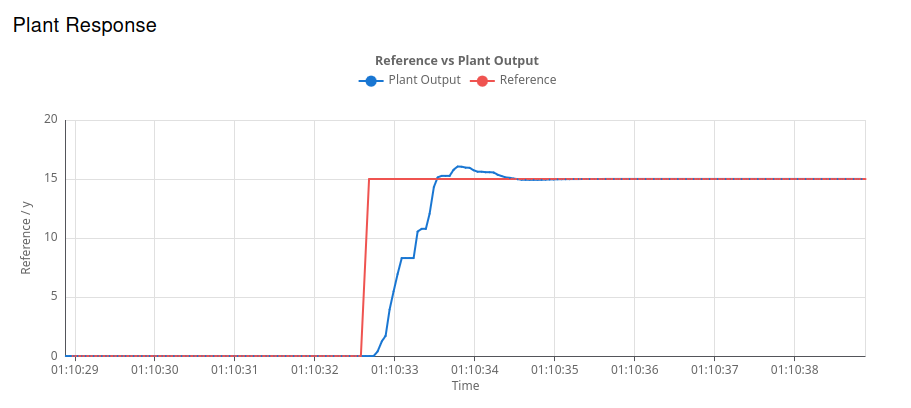
\includegraphics[width=\linewidth]{ensaio_v5_subida_planta.png}
        \caption{Aumento da referência.}
    \end{subfigure}
    \vspace{0.3cm}
    \begin{subfigure}{0.95\textwidth}
        \centering
        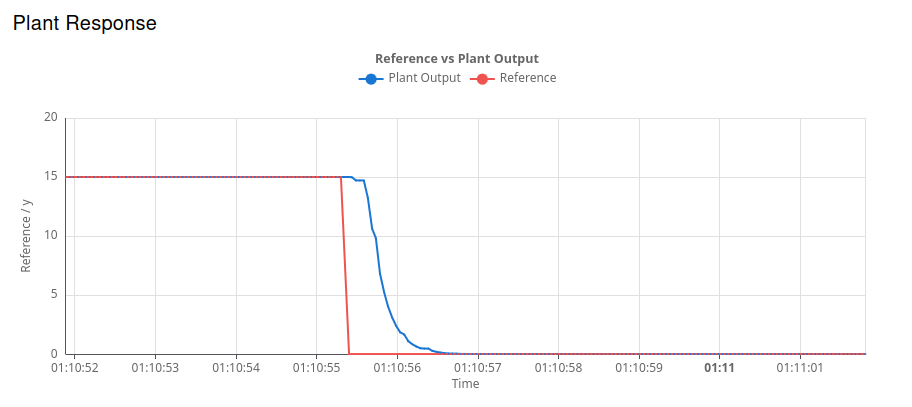
\includegraphics[width=\linewidth]{ensaio_v5_descida_planta.png}
        \caption{Redução da referência.}
    \end{subfigure}
    \caption{Rastreamento da referência para o vértice V5 ($\gamma_{ob}=0,040$, $\mu_m=0,10$ e $\mu_o=0,10$). Capturas do Node-RED.}
    \label{fig:ensaio_v5}
\end{figure}

Veja que para o vértice V4 a resposta ao aumento da referência ($0\rightarrow15$) não apresenta sobressinal visível. Na redução da referência ($15\rightarrow0$), a saída decresce e se aproxima novamente do valor solicitado, também sem oscilações significativas nas capturas apresentadas.

No entanto, para o vértice V5 o comportamento muda. No aumento da referência a saída ultrapassa o valor desejado de 15 e atinge um pico próximo de 16, antes de retornar à referência. Considerando que a amplitude do degrau de entrada é $\Delta y=15$, o sobressinal estimado é aproximadamente
\begin{equation}
    M_p=\frac{y_{\text{max}}-y_{\text{ss}}}{\Delta y}\approx\frac{16-15}{15}\times 100\%\approx 6,67\%.
    \label{eq:sobressinal_estimado}
\end{equation}

Da dashboard foi possível observar que a ação de controle também muda durante os degraus. A Figura~\ref{fig:controle_embarcado} apresenta os sinais $u$ para os dois ensaios de aumento da referência, evidenciando a diferença no transitório observado entre V4 e V5.

\begin{figure}[H]
    \centering
    \begin{subfigure}{0.95\textwidth}
        \centering
        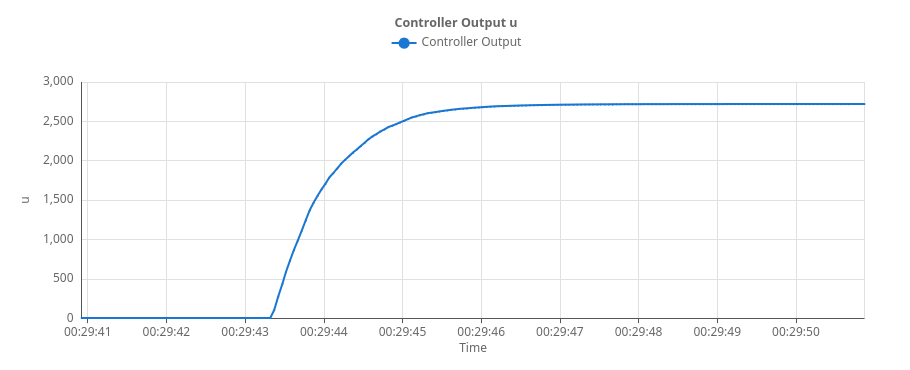
\includegraphics[width=\linewidth]{ensaio_v4_subida_controle.png}
        \caption{Ação de controle para o vértice V4.}
    \end{subfigure}
    \vspace{0.25cm}
    \begin{subfigure}{0.95\textwidth}
        \centering
        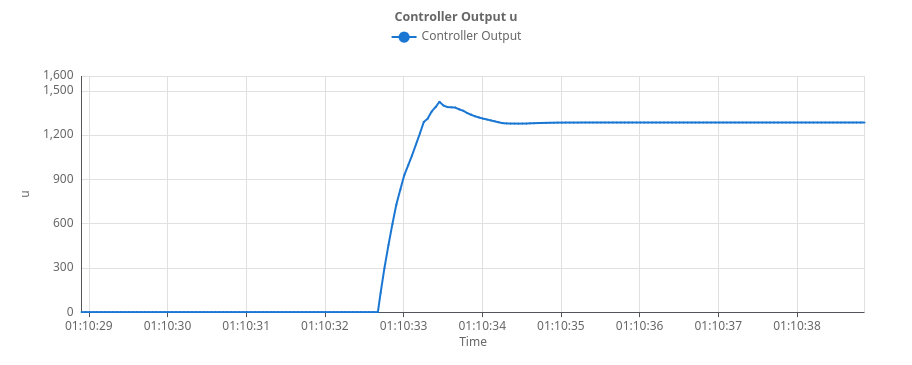
\includegraphics[width=\linewidth]{ensaio_v5_subida_controle.png}
        \caption{Ação de controle para o vértice V5.}
    \end{subfigure}
    \caption{Ação de controle registrada na dashboard durante o aumento da referência para os dois vértices V4 e V5.}
    \label{fig:controle_embarcado}
\end{figure}

Além destes ensaios também foram realizados testes, registrados em vídeo (\cite{maradiaga2026ensaio}),variando os parâmetros incertos do sistema por meio dos três potenciômetros conectados ao ESP32 planta.

\subsection{Discussão comparativa}
\label{subsec:discussao_comparativa}

Os testes realizados com o sistema embarcado mostram que, nas duas combinações paramétricas selecionadas, o controlador conseguiu conduzir a saída até a referência desejada. Observa-se, nas Figuras~\ref{fig:ensaio_v4} e~\ref{fig:ensaio_v5}, que as respostas transitórias foram diferentes entre os dois casos testados: V4 apresentou um comportamento semelhante ao de um sistema sobreamortecido, enquanto V5 apresentou um comportamento semelhante ao de um sistema subamortecido, devido à presença de sobressinal. Ao comparar as respostas da emulação com as simulações em Simulink, observa-se que, em ambas as implementações, a resposta sob V5 apresenta um tempo de estabilização ($t_s$) menor do que a resposta sob V4. No entanto, na emulação embarcada, a resposta do sistema sob os parâmetros de V5 apresenta sobressinal, diferentemente do observado na simulação. Essa diferença pode estar relacionada às características da implementação embarcada, como a latência introduzida pela temporização das tasks, a comunicação por UART entre os microcontroladores e o processamento dos sinais do ADC.

Além dos ensaios com parâmetros fixos, os testes realizados variando os parâmetros incertos durante a operação da malha mostraram que o controlador PI foi capaz de manter a estabilidade para algumas trajetórias de variação dos parâmetros dentro do politopo, sem necessidade de reajustar seus ganhos.

Portanto, os resultados experimentais complementam as simulações realizadas, mostrando que o controlador é capaz de manter a malha estável nas condições avaliadas, inclusive durante as alterações dos parâmetros da planta.



